\documentclass[11pt]{article}
% Shared preamble for the printable mini lessons (1.4 onward).
%   \documentclass[11pt]{article}
%   \input{../preamble}
% Build the key with:  pdflatex -jobname=<name>_KEY "\def\iskey{}\input{<name>}"
% Figures shared with the web page live in figures/Unit_X/<name>.tex and are
% pulled in with \fig{Unit_X/<name>}; the standalone package drops their own
% preamble, so their macros come from figures/preamble.tex, loaded here.
% Shared preamble for web figures.  Each figure is a standalone .tex that
% \input's this file; scripts/make-figures.sh turns it into an SVG.
\usepackage[T1]{fontenc}
\usepackage{helvet}
\renewcommand{\familydefault}{\sfdefault}
\usepackage{tikz}
\usetikzlibrary{decorations.pathreplacing}
% axis numbers in the text font, not math italic
\pgfkeys{/pgf/number format/.cd,assume math mode=true,1000 sep={}}

% dot plot: \dotplot{min}{max}{value/count,...}{axis label}
\newcommand{\dotplot}[4]{%
\begin{tikzpicture}[x=0.9cm,y=0.33cm]
  \draw[thick] (#1-0.5,0) -- (#2+0.5,0);
  \foreach \t in {#1,...,#2} {\draw (\t,0.25) -- (\t,-0.25) node[below] {\t};}
  \foreach \v/\c in {#3} {\ifnum\c>0 \foreach \k in {1,...,\c} {\fill (\v,\k*1.15) circle (0.16cm);}\fi}
  \node at ({(#1+#2)/2},-2.3) {#4};
\end{tikzpicture}}

% shape sketch histogram (12 bins): \shapehist{heights}{label}
\newcommand{\shapehist}[2]{%
  \foreach \h [count=\i from 0] in {#1} \draw[fill=gray!30] (\i,0) rectangle (\i+1,\h);
  \draw (-0.3,0) -- (12.3,0);
  \node[font=\bfseries] at (6,-2.6) {#2};}
\newcommand{\meanmark}[1]{\fill (#1,0) -- ++(-0.3,-0.75) -- ++(0.6,0) -- cycle;}
\newcommand{\medmark}[2]{\draw[very thick,dashed] (#1,0) -- (#1,#2);}

% number line with minor ticks: \nline{min}{max}{label step}{axis label}
\newcommand{\nline}[4]{%
  \draw[thick] (#1-0.5,0) -- (#2+0.5,0);
  \foreach \t in {#1,...,#2} \draw (\t,0.12) -- (\t,-0.12);
  \pgfmathtruncatemacro{\nxt}{#1+#3}
  \foreach \t in {#1,\nxt,...,#2} \draw (\t,0.2) -- (\t,-0.2) node[below] {\t};
  \node at ({(#1+#2)/2},-0.95) {#4};}
% box plot above the line: \bplot{min}{Q1}{med}{Q3}{max}
\newcommand{\bplot}[5]{%
  \draw[thick] (#1,1.0) -- (#2,1.0);
  \draw[thick] (#4,1.0) -- (#5,1.0);
  \draw[thick] (#1,0.75) -- (#1,1.25);
  \draw[thick] (#5,0.75) -- (#5,1.25);
  \draw[thick,fill=gray!20] (#2,0.55) rectangle (#4,1.45);
  \draw[very thick] (#3,0.55) -- (#3,1.45);}

% ---- added for 1.4 onward ----
% axis on y=0: \axis{min}{max}{label step}{tick step}{axis label}
\newcommand{\axis}[5]{%
  \draw[thick] (#1,0) -- (#2,0);
  \pgfmathsetmacro{\axT}{#1+#4}\foreach \t in {#1,\axT,...,#2} \draw (\t,0.1) -- (\t,-0.1);
  \pgfmathsetmacro{\axL}{#1+#3}\foreach \t in {#1,\axL,...,#2}
    \draw (\t,0.18) -- (\t,-0.18) node[below] {\pgfmathprintnumber{\t}};
  \node at ({(#1+#2)/2},-0.95) {#5};}
% box plot centred at height y: \bplotat{y}{min}{Q1}{med}{Q3}{max}
\newcommand{\bplotat}[6]{%
  \draw[thick] (#2,#1) -- (#3,#1);
  \draw[thick] (#5,#1) -- (#6,#1);
  \draw[thick] (#2,#1-0.22) -- (#2,#1+0.22);
  \draw[thick] (#6,#1-0.22) -- (#6,#1+0.22);
  \draw[thick,fill=gray!20] (#3,#1-0.42) rectangle (#5,#1+0.42);
  \draw[very thick] (#4,#1-0.42) -- (#4,#1+0.42);}
% an outlier dot: \outlier{x}{y}
\newcommand{\outlier}[2]{\fill (#1,#2) circle (2.4pt);}

\usepackage[margin=0.75in]{geometry}
\usepackage{array}
\usepackage{enumitem}
\usepackage{amsmath}
\usepackage[helvet]{sfmath}  % math in the same sans font as the text
\usepackage{standalone}
\pagestyle{empty}
\setlength{\parindent}{0pt}
\setlist[enumerate,1]{leftmargin=1.5em,itemsep=1em}
\setlist[enumerate,2]{label=(\alph*),leftmargin=2em,itemsep=2.2em}

\newif\ifkey
\ifdefined\iskey \keytrue \fi
\colorlet{keyred}{red!75!black}
\newcommand{\ans}[1]{\ifkey\leavevmode{\color{keyred}#1}\fi}
% vertical work space on the student copy, less on the key
\newcommand{\work}[1]{\ifkey\vspace{0.6em}\else\vspace{#1}\fi}
\newcommand{\fig}[1]{\input{../../figures/#1}}
% Title line: \lessontitle{Quartiles, IQR, and Box Plots}
\newcommand{\lessontitle}[1]{{\Large\bfseries #1\ifkey\ \textcolor{keyred}{KEY}\fi}\hfill Name \underline{\hspace{2in}}\par\vspace{0.6em}}
\newcommand{\partner}{\par\vspace{0.4em}Work with a partner. Compare answers when you finish each problem.\par}

% Unit quiz: two questions per mini lesson, each headed by the lesson's
% objective.  The key keeps every box the same height as the student copy,
% so key page N lines up with quiz page N.
\newcommand{\lessonhead}[1]{\par\vspace{0.6em}{\large\bfseries #1}\par\vspace{0.25em}\hrule\vspace{0.6em}}
\newcommand{\goal}[1]{\textbf{#1}\par\vspace{0.35em}}
% answer box: same height on both copies, answer printed only on the key
\newcommand{\abox}[2]{\par\begin{minipage}[t][#1][t]{\linewidth}\raggedright\vspace{0.2em}\ans{#2}\end{minipage}\par}
% circled choices: \opt{A} prints plain; \optans{B} is circled in red on the key
\newcommand{\opt}[1]{\tikz[baseline=(c.base)]\node[rounded corners=0.6em,inner sep=2.5pt](c){#1};}
\newcommand{\optans}[1]{\ifkey\tikz[baseline=(c.base)]\node[rounded corners=0.6em,inner sep=2.5pt,draw=keyred,thick,text=keyred](c){#1};\else\opt{#1}\fi}
% r blank under a scatterplot, filled in red on the key
\newcommand{\rblank}[1]{\underline{\makebox[0.6in]{\ans{#1}}}}
\setlist[enumerate,2]{label=(\alph*),leftmargin=2em,itemsep=0.3em}
\setlist[enumerate,1]{leftmargin=1.5em,itemsep=1em}
\raggedright\hyphenpenalty=10000\exhyphenpenalty=10000

\begin{document}

\lessontitle{Unit 4 Quiz: Scatterplots}

Show your work.

% ======================================================================
\lessonhead{4.1 - Scatterplots and Lines of Best Fit}
\begin{enumerate}

\item \goal{I describe the direction, form, and strength of a scatterplot, and I choose a good line of best fit.}
A store counted the people ahead of 10 customers in line and timed each wait.

\vspace{0.3em}
\renewcommand{\arraystretch}{1.1}
\begin{tabular}{|l|*{10}{c|}}\hline
People ahead in line ($x$) & 1 & 2 & 3 & 4 & 5 & 6 & 8 & 9 & 10 & 12 \\ \hline
Minutes waited ($y$) & 7 & 5 & 12 & 10 & 10 & 17 & 17 & 22 & 26 & 24 \\ \hline
\end{tabular}

\vspace{0.5em}
\begin{minipage}[t]{0.44\linewidth}\vspace{0pt}\raggedright
\begin{tikzpicture}[x=0.48cm,y=0.105cm]
  \grid{0}{12}{1}{0}{30}{5}{People ahead in line}{Minutes waited}
  \pts{1/7,2/5,3/12,4/10,5/10,6/17,8/17,9/22,10/26,12/24}
  \ifkey\draw[keyred,thick] (0,3) -- (12,27);\fi
\end{tikzpicture}
\end{minipage}\hfill
\begin{minipage}[t]{0.54\linewidth}\vspace{0pt}\raggedright
\begin{enumerate}
  \item Describe the direction, form, and strength.
  \abox{2em}{Positive, linear, strong}
  \item Draw a line of best fit on the graph.
  \abox{2.8em}{One good line is in red. Accept any line through the middle of the dots.}
  \item How many dots are above your line? How many are below?
  \abox{2em}{Red line: 5 above and 5 below}
\end{enumerate}
\end{minipage}

\item \goal{I write the equation of a line of best fit, and I make predictions and know when not to trust them.}
A school sells hot chocolate at football games. The scatterplot shows the temperature and the number of cups sold at 10 games. A line of best fit is drawn.

\vspace{0.3em}
\begin{minipage}[t]{0.42\linewidth}\vspace{0pt}\raggedright
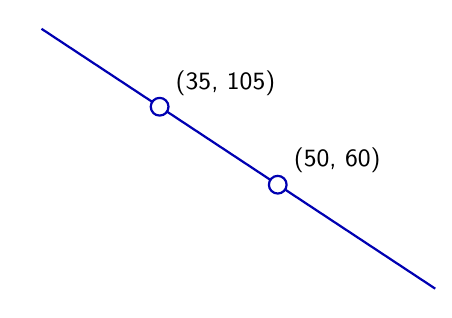
\begin{tikzpicture}[x=0.1cm,y=0.022cm]
  \grid{20}{70}{5}{0}{160}{20}{Temperature ($^\circ$F)}{Cups sold}
  \draw[thick,blue!70!black] (20,150) -- (70,0);
  \pts{25/141,30/115,32/118,38/90,40/93,45/71,48/71,55/42,60/35,65/10}
  \foreach \p in {(35,105),(50,60)} \draw[thick,blue!70!black,fill=white] \p circle (3.2pt);
  \node[font=\small,anchor=south west] at (35.8,106) {(35, 105)};
  \node[font=\small,anchor=south west] at (50.8,61) {(50, 60)};
\end{tikzpicture}
\end{minipage}\hfill
\begin{minipage}[t]{0.56\linewidth}\vspace{0pt}\raggedright
\begin{enumerate}
  \item Use the two marked points to find the slope.
  \abox{3.4em}{$m = \frac{60 - 105}{50 - 35} = \frac{-45}{15} = -3$}
  \item Write the equation of the line.
  \abox{4.4em}{$105 = -3(35) + b$\\ $105 = -105 + b$, \; so $b = 210$\\[0.3em] $\hat{y} = -3x + 210$}
\end{enumerate}
\end{minipage}

\vspace{0.4em}
\begin{minipage}[t]{0.4\linewidth}\vspace{0pt}\raggedright
\begin{enumerate}[start=3]
  \item Predict the number of cups sold when the temperature is 42$^\circ$F.
  \abox{4.2em}{$\hat{y} = -3(42) + 210$\\ $= -126 + 210 = 84$ cups}
\end{enumerate}
\end{minipage}\hfill
\begin{minipage}[t]{0.58\linewidth}\vspace{0pt}\raggedright
\begin{enumerate}[start=4]
  \item Predict the number of cups sold when the temperature is 80$^\circ$F. Does your answer make sense? Explain.
  \abox{4em}{$\hat{y} = -3(80) + 210 = -30$. No. A school cannot sell fewer than 0 cups. 80$^\circ$F is far outside the data (25$^\circ$F to 65$^\circ$F).}
\end{enumerate}
\end{minipage}

\end{enumerate}

% ======================================================================
\newpage
\lessonhead{4.2 - Slope, Intercept, and Correlation}
\begin{enumerate}[resume]

\item \goal{I explain the slope of a line of best fit in context, and I explain the y-intercept in context, or tell why it has no meaning.}
A coach recorded how many hours each player practiced last week and how many free throws each player made out of 50. The line of best fit is $\hat{y} = 2x + 15$.
\begin{enumerate}
  \item Explain the slope in context.
  \abox{3.6em}{For each additional hour of practice, the predicted number of free throws made increases by 2.}
  \item Explain the y-intercept in context.
  \abox{3.6em}{When $x = 0$ (no practice), the predicted number of free throws made is 15.}
\end{enumerate}

\vspace{0.3em}
A bookstore uses the line $\hat{y} = 0.03x + 4$, where $x$ is the number of pages in a book and $y$ is the price in dollars.
\begin{enumerate}[start=3]
  \item Does the y-intercept have a real meaning here? Explain.
  \abox{3.6em}{No. It says a book with 0 pages costs \$4. No book has 0 pages.}
\end{enumerate}

\item \goal{I estimate the correlation coefficient $r$ from a scatterplot, and I explain why correlation does not prove causation.}
\begin{enumerate}
  \item Match each $r$ to a scatterplot: \quad $r = -0.9$, \; $r = 0.2$, \; $r = 0.7$

  \vspace{0.5em}
  \begin{tikzpicture}[x=0.32cm,y=0.32cm]
    \foreach \lab/\sx in {A/0,B/14,C/28} {
      \begin{scope}[shift={(\sx,0)}]
        \draw[thick] (0,0) -- (10,0); \draw[thick] (0,0) -- (0,10);
        \node[font=\bfseries] at (5,11) {\lab};
      \end{scope}}
    % A: r = 0.7, B: r = -0.9, C: r = 0.2
    \begin{scope}[shift={(0,0)}]\pts{0.8/3.4,1.6/4.0,2.2/3.5,3.3/3.0,3.9/4.6,4.4/2.6,4.7/4.1,5.5/6.6,6.1/7.7,6.9/6.4,7.6/3.5,8.3/8.1,9.0/7.5}\end{scope}
    \begin{scope}[shift={(14,0)}]\pts{0.8/7.5,1.8/7.8,2.6/7.1,2.8/7.8,3.6/5.0,4.2/5.1,4.7/4.5,5.9/2.8,6.3/4.2,6.8/4.2,7.8/2.3,8.2/3.9,9.2/2.7}\end{scope}
    \begin{scope}[shift={(28,0)}]\pts{1.2/2.5,1.6/4.0,2.3/6.4,2.9/5.6,3.8/4.1,4.5/7.7,5.1/1.9,5.8/5.3,6.5/5.5,6.9/8.6,7.6/3.7,8.2/3.3,9.2/6.5}\end{scope}
    \foreach \lab/\sx in {A/0,B/14,C/28} \node[anchor=base] at (\sx+5,-2.2) {$r = $ \rblank{}};
    \ifkey
      \node[anchor=base,keyred] at (5.9,-2.1) {$0.7$};
      \node[anchor=base,keyred] at (19.9,-2.1) {$-0.9$};
      \node[anchor=base,keyred] at (33.9,-2.1) {$0.2$};
    \fi
  \end{tikzpicture}

  \vspace{0.8em}
  \item In many cities, the number of fast food restaurants and the number of schools have a strong positive correlation. Which statement is true? Circle the letter.

  \vspace{0.3em}
  \begin{tabular}{@{}l>{\raggedright\arraybackslash}p{5.6in}}
  \opt{A} & Building more fast food restaurants causes a city to have more schools.\\
  \opt{B} & Building more schools causes a city to have more fast food restaurants.\\
  \optans{C} & A lurking variable, such as the number of people in the city, could cause both.\\
  \opt{D} & There is no relationship, because restaurants and schools are different things.\\
  \end{tabular}
\end{enumerate}

\end{enumerate}

% ======================================================================
\newpage
\lessonhead{4.3 - Residuals}
\begin{enumerate}[resume]

\item \goal{I find and explain a residual, and I tell if a point is above or below the line from its residual.}
A taxi company predicts the fare with $\hat{y} = 2.5x + 4$, where $x$ is the distance in miles and $y$ is the fare in dollars.
\begin{enumerate}
  \item Fill in the table.

  \vspace{0.3em}
  \renewcommand{\arraystretch}{1.6}
  \begin{tabular}{|c|c|p{1.35in}|p{1.35in}|}\hline
  $x$ (miles) & $y$ (actual fare) & $\hat{y}$ (predicted) & residual $y - \hat{y}$ \\ \hline
  2 & 10 & \ans{$2.5(2) + 4 = 9$} & \ans{$10 - 9 = 1$} \\ \hline
  4 & 13 & \ans{$2.5(4) + 4 = 14$} & \ans{$13 - 14 = -1$} \\ \hline
  6 & 20 & \ans{$2.5(6) + 4 = 19$} & \ans{$20 - 19 = 1$} \\ \hline
  8 & 22 & \ans{$2.5(8) + 4 = 24$} & \ans{$22 - 24 = -2$} \\ \hline
  \end{tabular}
  \item Which rides have points above the line? How do you know?
  \abox{2.6em}{The 2-mile and 6-mile rides. Their residuals are positive.}
  \item Explain the residual for the 8-mile ride in context.
  \abox{2.6em}{The residual is $-2$. The fare was \$2 less than predicted.}
\end{enumerate}

\item \goal{I explain what the least-squares line is, and I use a residual plot to decide if a line is a good model.}
Two lines were fit to the same 4 points. Here are their residuals.

\vspace{0.3em}
\begin{minipage}[t]{0.53\linewidth}\vspace{0pt}\raggedright
\renewcommand{\arraystretch}{1.6}
\begin{tabular}{|l|c|c|c|c|p{1.3in}|}\hline
 & \multicolumn{4}{c|}{Residuals} & $\Sigma(y - \hat{y})^2$ \\ \hline
Line A & 2 & $-3$ & 1 & 0 & \ans{$4 + 9 + 1 + 0 = 14$} \\ \hline
Line B & $-1$ & 2 & $-2$ & 1 & \ans{$1 + 4 + 4 + 1 = 10$} \\ \hline
\end{tabular}
\end{minipage}\hfill
\begin{minipage}[t]{0.44\linewidth}\vspace{0pt}\raggedright
\begin{enumerate}
  \item Find $\Sigma(y - \hat{y})^2$ for each line. Write it in the table.
  \item Which line is closer to the least-squares line? Explain.
  \abox{3.8em}{Line B. Its sum of squared residuals (10) is smaller than Line A's (14).}
\end{enumerate}
\end{minipage}

\vspace{0.3em}
\begin{minipage}[t]{0.36\linewidth}\vspace{0pt}\raggedright
\begin{tikzpicture}[x=0.45cm,y=0.5cm]
  \draw[thick] (0,-2.6) -- (0,2.6); \draw[thick,dashed] (0,0) -- (11,0);
  \node[left,font=\small] at (0,0) {0};
  \node[rotate=90,font=\small] at (-1.3,0) {residual};
  \node[below,font=\small] at (5.5,-2.6) {$x$};
  \pts{1/-1.1,2/0.6,3/1.8,4/-0.5,5/-1.6,6/0.9,7/-0.2,8/1.4,9/-1.7,10/0.4}
\end{tikzpicture}
\end{minipage}\hfill
\begin{minipage}[t]{0.61\linewidth}\vspace{0pt}\raggedright
\begin{enumerate}[start=3]
  \item This is the residual plot for a line of best fit for another data set. Which statement is true? Circle the letter.

  \vspace{0.3em}
  \begin{tabular}{@{}l>{\raggedright\arraybackslash}p{3.3in}}
  \optans{A} & A line is a good model, because the residuals show no pattern.\\
  \opt{B} & A line is not a good model, because some residuals are negative.\\
  \opt{C} & A line is not a good model, because the residuals are not all 0.\\
  \opt{D} & A line is a good model, because the residuals make a curved pattern.\\
  \end{tabular}
\end{enumerate}
\end{minipage}

\end{enumerate}

\end{document}
